The area of the smallest equilateral triangle with one vertex on each of the sides of the right triangle with side lengths $2\sqrt3$, $5$, and $\sqrt{37}$, as shown, is $\tfrac{m\sqrt{p}}{n}$, where $m$, $n$, and $p$ are positive integers, $m$ and $n$ are relatively prime, and $p$ is not divisible by the square of any prime. Find $m+n+p$.
\begin{center}
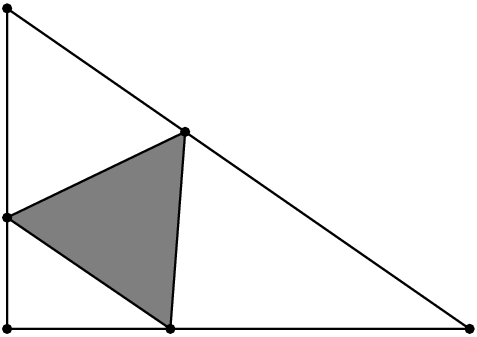
\includegraphics[width = 47.6mm]{img/fig0.png}
\end{center}